\subsection{Observations on intervals, fibers, and rectangles}\label{macro:observaciones}

Take a partition $\mathcal I$ of $[0,1]$ into intervals of length at most $a_{\rm mac}$, assigning
each endpoint to a single interval. We may take all intervals to have equal length. An index belongs
to the interval containing its physical center. For rows and columns we record
\[
 N^R_I=\frac1n\sum_{r_i\in I}X_{R_i},\qquad
 N^C_I=\frac1n\sum_{c_j\in I}X_{C_j},\qquad
 N^{R,*}_I=N^{C,*}_I=x|I|.
\]
The fiber parameter is $c$ on a row and $r$ on a column, diagonal, or antidiagonal. Fix a line
$\lambda$, called the \emph{tracked line}, whose fiber we observe. For an interval $I$, write
$\lambda_I$ for the part of the physical fiber whose parameter belongs to $I$, and $dz$ for the
parameter measure. There is no Euclidean length factor on oblique fibers, since there are $n$
indices per unit of $r$.

\begin{definicion}[Fiber observations]\label{macro:fibras}
While $\lambda$ is available, its observation is
\[
 F_{\lambda,I}=\frac1n\sum_{e\in\lambda_I}
                  \prod_{f\ni e,\ f\ne\lambda}X_f .
\]
For each of the four families, the target $F^*_{\lambda,I}$ is the integral over $\lambda_I$ of the
density in the second column of the table. The last column gives the sum of the rates for the three
lines in the product, before division by $x$.
\[
\begin{array}{c|c|c}
 \lambda & \text{target density} & H^*_{\lambda}(e)\\ \hline
 R_i & xU_DU_A  & 1+\ell_D^*+\ell_A^*\\
 C_j & xU_DU_A  & 1+\ell_D^*+\ell_A^*\\
 D_d & x^2U_A   & 2+\ell_A^*\\
 A_{a'} & x^2U_D & 2+\ell_D^*
\end{array}
\]
If the choice at a step occupies $\lambda$, we retain the values of $F_{\lambda,I}$ and
$F^*_{\lambda,I}$ immediately before that step and hold them constant thereafter. We call this the
\emph{freezing rule}. The balances in Lemma~\ref{macro:balances} use only lines that are still
available.
\end{definicion}

Order the positions of a rectangle as
$e_1=(i,j)$, $e_2=(i',j)$, $e_3=(i',j')$, $e_4=(i,j')$.
Call a quadruple $(i,i',j,j')$ ordinary if $i\ne i'$, $j\ne j'$, and the four labels within each
diagonal family are pairwise distinct. There are $O(n^3)$ remaining quadruples. Each forbidden
equality is a nontrivial linear equation in four indices. Fixing three suitably chosen indices
determines the fourth, and there are only a fixed number of equalities. This estimate also covers
the edges of the board.

\begin{definicion}[Rectangle observations]\label{macro:rectangulos}
For $T\subseteq\{1,2,3,4\}$ and a box $\Theta\in\mathcal I^4$, we track the sum and its target
\begin{align*}
 P_{\Theta,T}&=\frac1{n^4}
 \sum_{(i,i',j,j')\in\Theta}^{\rm ord}
 X_{R_i}X_{R_{i'}}X_{C_j}X_{C_{j'}}
 \prod_{m\in T}X_{D(e_m)}X_{A(e_m)},\\
 P^*_{\Theta,T}&=\int_\Theta x^4\prod_{m\in T}U_{D(e_m)}U_{A(e_m)}
                  \,dr\,dr'\,dc\,dc'.
\end{align*}
The four continuous coordinates determine the positions in the integral. The pattern for
$T=\varnothing$ counts only the two rows and two columns. Individual rectangles cease to contribute
when they lose a line.
\end{definicion}

We measure the discrepancies by
\begin{align*}
 \Delta_0&=\sum_{I\in\mathcal I}
   (\bigl|N^R_I-x|I|\bigr|+\bigl|N^C_I-x|I|\bigr|),\\
 \Delta_F&=\max_{\lambda}\sum_{I\in\mathcal I}|F_{\lambda,I}-F^*_{\lambda,I}|,\\
 \Delta_R&=\sum_{\Theta\in\mathcal I^4}\ \sum_{T\subseteq\{1,2,3,4\}}
                      |P_{\Theta,T}-P^*_{\Theta,T}|,\qquad
 \Delta=\Delta_0+\Delta_F+\Delta_R .
\end{align*}
In the first line, $x|I|$ is the target mass of each interval. We write $C_{\mathcal I}$ for constants
that may depend on the fixed partition $\mathcal I$, and set
\[
 \zeta=\Delta_0+\Delta_F+a_{\rm mac}+C_{\mathcal I}/n .
\]
On the $k$ available rows and $k$ available columns, consider
\[
 q_{ij}=\frac{Y_{ij}\nu_1(r_i,c_j)}{kU_{D(i,j)}U_{A(i,j)}},\qquad
 V_{ij}=\frac{\nu_1(r_i,c_j)}k .
\]
The factors $U$ are evaluated at $x$, so $q_{ij}=Y_{ij}W_x(r_i,c_j)/k=Y_{ij}v_x(r_i,c_j)/n$.
The matrix $q$ is our explicit candidate for the Bethe point. Proposition~\ref{macro:maximo} proves
that $p_e/q_e$ is close to one on available squares. Replacing $Y_{ij}$ in $q$ by $U_DU_A$, its
target when the row and column are available, gives the matrix $V$.

Figure~\ref{fig:rectangulo} shows two selected positions and their corresponding sign.
\begin{figure}[htbp]
\centering
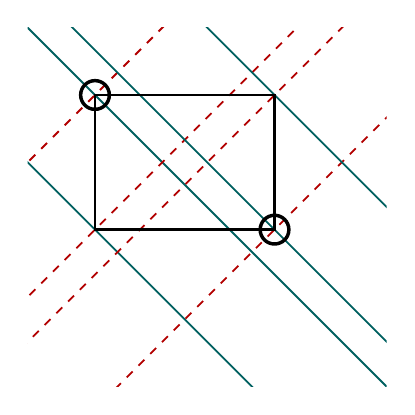
\begin{tikzpicture}[x=.57cm,y=.57cm]
 \bcuadricula{8}
 \begin{scope}
  \clip (0,0) rectangle (8,8);
  \foreach \rr/\cc in {2/2,5/2,5/6,2/6}{
   \draw[teal!75!black,line width=.65pt] ({\cc-.5},{8.5-\rr}) ++(-8,8) -- ++(16,-16);
   \draw[red!70!black,dashed,line width=.65pt] ({\cc-.5},{8.5-\rr}) ++(-8,-8) -- ++(16,16);
  }
 \end{scope}
 \draw[black,line width=1pt] (1.5,6.5) rectangle (5.5,3.5);
 \foreach \rr/\cc in {2/2,5/2,5/6,2/6}{\bmarca{8}{\rr}{\cc}}
 \draw[black,line width=1.25pt] (1.5,6.5) circle[radius=.32];
 \draw[black,line width=1.25pt] (5.5,3.5) circle[radius=.32];
\end{tikzpicture}
\caption{A rectangle on an empty board of order eight. Rows are numbered from one, top to bottom,
and columns from one, left to right. The vertices, in order, are $e_1=(2,2)$, $e_2=(5,2)$,
$e_3=(5,6)$ and $e_4=(2,6)$. Four diagonals $i-j$ (solid) and four antidiagonals $i+j-1$ (dashed)
pass through them. The circles select the opposite vertices $e_1,e_3$. The term in the expansion with
$T=\{1,3\}$ has sign $(-1)^{4-2}=+1$.}\label{fig:rectangulo}
\end{figure}


\begin{lema}[Interval and fiber balances]\label{macro:balances}
For $k\ge\delta n$, the row and column sums of $V$ differ from one by
$O_\delta(\Delta_0+a_{\rm mac}+C_{\mathcal I}/n)$. For $q$, the row and column sums differ from one
and the masses on available diagonal lines differ from $\ell_f^*$ by
$O_\delta(\Delta_F+a_{\rm mac}+C_{\mathcal I}/n)$, uniformly over the lines.
\end{lema}
\begin{proof}
On each interval we replace the weight by its value at a point of the physical region of integration.
The weights $\nu_1$ and $W_x=\nu_1/(U_DU_A)$ are uniformly bounded and Lipschitz. The error of this
replacement, summed over the intervals of a line, is $O_\delta(a_{\rm mac})$, since the variation in
the weight multiplies the sum of the masses on that line. The error in the weighted masses is at
most the supremum norm of the weight times the sum of the absolute discrepancies. Converting $1/n$
to $1/k$ contributes a factor $1/x$. For $V$, the target for a row is
$x^{-1}\int\nu_1(r,c)x\,dc=1$, and the same holds for columns. On an available row, the three
indicators in the fiber observable give $Y_{ij}$, and its target weighted mass is
\[
 \frac1x\int_0^1 \frac{\nu_1}{U_DU_A}\,xU_DU_A\,dc=1.
\]
The same calculation with $dr$ gives the column sum. For diagonal $d$, the target is
\[
 \frac1x\int_{D_d}\frac{\nu_1}{U_DU_A}\,x^2U_A\,dr
 =\frac{xm_D(d)}{U_D(d)} .
\]
Interchanging $D$ and $A$ for an antidiagonal gives $xm_A/U_A$. Endpoint or Riemann sum
approximations on the fixed partition incur an error of at most $C_{\mathcal I}/n$.
\end{proof}
